\section{Dinamica Manipolatore}
Il modello dinamico del manipolatore ci fornisce una descrizione matematica della relazione che è instaurata tra le forze agenti sul robot (generalizzate) ed il movimento prodotto dalla sua struttura, cioè le configurazioni che assume nel tempo. Inizialmente, nel calcolo della dinamica sono stati usati tre metodi diversi, il metodo delle azioni vincolari, il metodo di Lagrange e quello dei lavori virtuali. Si è poi deciso di proseguire esclusivamente con il PLV. L'obiettivo di questa sezione è quello di mostrare l'approccio e i risultati ottenuti per il calcolo della dinamica diretta ed inversa.
\subsection{Prerequisiti per il calcolo della dinamica}\label{sec:prerequisiti-dinamica}
Prima di andare ad analizzare i metodi utilizzati, è importante andare a ricavare tutte le matrici delle quali avremo bisogno, in particolare è necessario andare a definire delle matrici che ci permettano di ottenere $\theta_3$ e $\theta_4$ in funzione di $\theta_1$ e $\theta_2$.
\subsubsection{Jacobiana $J_{34}$ e calcolo $\dot{\theta_3},\dot{\theta_4}$}
A partire da $\theta_1, \theta_2$ possiamo, mediante la cinematica diretta ottenere $\theta_3$ e $\theta_4$, unendo queste quattro componenti e considerando anche le velocità $\dot{\theta_1}$ e $\dot{\theta_2}$ possiamo andare a ricavare la matrice $J_{34}$ che esprime $\theta_3$ e $\theta_4$ in funzione di $\theta_1, \theta_2$ e possiamo ricavare anche $\dot{\theta_3}, \dot{\theta_4}$, per far questo andiamo a definire le seguenti quantità:
\begin{equation*}
    N_{13} = \frac{\cos\theta_4}{\sin\theta_4}\sin\theta_1-\cos\theta_1
\end{equation*}
\begin{equation*}
    N_{23} = \cos\theta_2-\frac{\cos\theta_4}{\sin\theta_4}\sin\theta_2
\end{equation*}
\begin{equation*}
    D_{13} = \cos\theta_3-\frac{\cos\theta_4}{\sin\theta_4}\sin\theta_3
\end{equation*}
Da queste tre formule possiamo andare a ricavare $\dot{\theta_3}$ nel seguente modo:
\begin{equation}
    \dot{\theta_3} = \frac{\dot{\theta_1}N_{13}}{D_{13}}+\frac{\dot{\theta_2}N_{23}}{D_{13}}
\end{equation}
Proseguiamo ora definendo le equazioni che ci serviranno per calcolare $\dot{\theta_4}$:
\begin{equation*}
    N_{14} = \frac{\sin\theta_1\cos\theta_3}{\sin\theta_3}-\frac{\cos\theta_4}{\sin\theta_4}+\frac{\cos\theta_4}{\sin\theta_4}\sin\theta_1 - \cos\theta_1
\end{equation*}
\begin{equation*}
    N_{24} = -\frac{\sin\theta_2\cos\theta_3}{\sin\theta_3}-\frac{\cos\theta_4}{\sin\theta_4}-\frac{\cos\theta_4}{\sin\theta_4}\sin\theta_2+\cos\theta_2
\end{equation*}
\begin{equation*}
    D_{14} = \frac{\sin\theta_4\cos\theta_3}{\sin\theta_3}-\frac{\cos\theta_4}{\sin\theta_4}
\end{equation*}
Otteniamo quindi:
\begin{equation}
    \dot{\theta_4} = \dot{\theta_1}\frac{N_{14}}{D_{14}}+\dot{\theta_2}\frac{N_{24}}{D_{14}}
\end{equation}
Il passo finale è quello di andare a rappresentare la matrice jacobiana che lega le velocità $\dot{\theta_3}$ e $\dot{\theta_4}$ con le velocità in ingresso al manipolatore:
\begin{equation}
    J_{34} = \begin{bmatrix}
    \frac{N_{13}}{D_{13}} & \frac{N_{23}}{D_{13}} \\
    \frac{N_{14}}{D_{14}} & \frac{N_{24}}{D_{14}}
    \end{bmatrix}
\end{equation}
%Notiamo che possiamo esprimere i parametri appena calcolati anche come:
%\begin{equation*}
%	\begin{bmatrix}
%		\dot{\theta_3} \\ \dot{\theta_4}
%	\end{bmatrix} = J_{34}\begin{bmatrix}
%	\dot{\theta_1} \\ \dot{\theta_2}
%\end{bmatrix}
%\end{equation*}
\subsubsection{Jacobiana $\dot{J_{34}}$ e calcolo di $\ddot{\theta_3}, \ddot{\theta_4}$}
Per andar ad ottenere la jacobiana finale, ed i valori delle accelerazioni sui link distali occorre derivare tutti gli elementi visti in precedenza, in particolare:
\begin{equation*} %  N11p =  N13p
    \dot{N_{13}} = \frac{-1}{\sin^2\theta_4\cdot\dot{\theta_4}\sin\theta_1}+\frac{\cos\theta_4}{\sin\theta_4}\cos\theta_1\dot{\theta_1}+\sin\theta_1\dot{\theta_1}
\end{equation*}
\begin{equation*} %N12p = N23p
   \dot{N_{23}} =\frac{1}{\sin^2\theta_4\cdot\dot{\theta_4}\sin\theta_2}-\frac{\cos\theta_4}{\sin\theta_4}\cos\theta_2\dot{\theta_2}-\sin\theta_2\dot{\theta_2}
\end{equation*}
\begin{equation*} % D1p = D13p
  \dot{D_{13}} =  -\sin\theta_3\dot{\theta_3} + \frac{1}{\sin^2\theta_4}\dot{\theta_4}\sin\theta_3 -\frac{ \cos\theta_4} {\sin\theta_4}\cos\theta_3\dot{\theta_3}
\end{equation*}
\begin{equation*} % N21p = N14p
\begin{aligned}
    \dot{N_{14}} = \cos\theta_1\dot{\theta_1}\bigg(\frac{\cos\theta_3}{\sin\theta_3}-\frac{\cos\theta_4}{\sin\theta_4}\bigg) + \sin\theta_1\bigg(\frac{1}{\sin^2\theta_3}\dot{\theta_3}+\frac{1}{\sin^2\theta_4}\dot{\theta_4}\bigg)+\\+\frac{-1}{\sin^2\theta_4}\dot{\theta_4}\sin\theta_1 +\cot\theta_4\cos\theta_1\dot{\theta_1}+\sin\theta_1\dot{\theta_1}
    \end{aligned}
\end{equation*}
\begin{equation*} % N22p = N24p
    \begin{aligned}
    \dot{N_{24}} = -\cos\theta_2\dot{\theta_2}\bigg(\frac{\cos\theta_3}{\sin\theta_3} - \frac{\cos\theta_4}{\sin\theta_4} \bigg) - \sin\theta_2\bigg(\frac{-1}{\sin^2\theta_3}\dot{\theta_3} + \frac{1}{\sin^2\theta_4}\dot{\theta_4}\bigg) -\\
    - \frac{-1}{\sin^2\theta_4}\dot{\theta_4}\sin\theta_2-\cot\theta_4\cos\theta_2\dot{\theta_2}-\sin\theta_2\dot{\theta_2}
    \end{aligned}
\end{equation*}
\begin{equation*} % D2p = D14p
   \dot{D_{14}} = \cos\theta_4\dot{\theta_4}(\cot\theta_3-\cot\theta_4)+\sin\theta_4\bigg(\frac{-1}{\sin^2\theta_3}\dot{\theta_3} + \frac{1}{\sin^2\theta_4}\dot{\theta_4}\bigg)
\end{equation*}
Esprimendo la matrice jacobiana $\dot{J_{34}}$ in funzione dei parametri appena trovati scriviamo:
\begin{equation}
    \dot{J_{34}} =
    \begin{bmatrix}
    \frac{\dot{N_{13}}D_{13}-N_{13}\dot{D_{13}}}{D_{13}^2} & 
     \frac{\dot{N_{23}}D_{13}-N_{23}\dot{D_{13}}}{D_{13}^2} \\
    \frac{\dot{N_{14}}D_{14}-N_{14}\dot{D_{14}}}{D_{14}^2} &
     \frac{\dot{N_{24}}D_{14}-N_{24}\dot{D_{14}}}{D_{14}^2}
    \end{bmatrix}
\end{equation}
Per concludere andiamo a trovare:
\begin{equation}
    \begin{bmatrix}
    \ddot{\theta_3} \\ \ddot{\theta_4}
    \end{bmatrix}
    = 
    \dot{J_{34}}\begin{bmatrix}
    \dot{\theta_1} \\ \dot{\theta_2}
    \end{bmatrix} + 
    J_{34} \begin{bmatrix}
    \ddot{\theta_1} \\ \ddot{\theta_2}
    \end{bmatrix}
\end{equation}
\subsubsection{Matrici di inerzia}
Per trovare la soluzione all'equazione del PLV introduciamo le matrici che hanno avuto un ruolo fondamentale nel calcolo:
\begin{equation*}
    J_1 = \begin{bmatrix}
     -0.5l\sin\theta_1 & 0 \\ 0.5l\cos\theta_1 & 0
    \end{bmatrix} \Rightarrow
    \dot{J_1} = \begin{bmatrix}
     -0.5l\cos\theta_1\dot{\theta_1} & 0 \\ -0.5l\sin\theta_1\dot{\theta_1} & 0
    \end{bmatrix}
\end{equation*}
\begin{equation*}
    J_2 = \begin{bmatrix}
           0 & -0.5*l*\sin\theta_2 \\
           0 & 0.5*l*\cos\theta_2 
           \end{bmatrix}
           \Rightarrow
   \dot{J_2} = \begin{bmatrix} 0 & -0.5l\cos\theta_2\dot{\theta_2} \\
           0 & -0.5l\sin\theta_2\dot{\theta_2}
           \end{bmatrix}
\end{equation*}
\begin{equation*}
    J_3 = \begin{bmatrix}
    -l\sin\theta_1+0.5\sin\theta_3\cdot J_{34}(1,1) & 
    -0.5l\sin\theta_3\cdot J_{34}(1,2) \\
    l\cos\theta_1+0.5\cos\theta_3\cdot J_{34}(1,1) & 
    0.5l\cos\theta_3\cdot J_{34}(1,2)
    \end{bmatrix}
\end{equation*}
\begin{equation*}
    J_4 = \begin{bmatrix}
    -0.5l\sin\theta_4\cdot J_{34}(2,1) &
    -l\sin\theta_2+0.5\sin\theta_4\cdot J_{34}(2,2) \\
    0.5l\cos\theta_4\cdot J_{34}(2,1) &
    l\cos\theta_2+0.5\cos\theta_4\cdot J_{34}(2,2)
    \end{bmatrix}
\end{equation*}
\begin{equation*}
    J_E = \begin{bmatrix}
    -l(\sin\theta_1+\sin\theta_3\cdot J_{34}(1,1)) & 
    -l\sin\theta_3 \cdot J_{34}(1,2) \\
    l(\cos\theta_1+\cos\theta_3\cdot J_{34}(1,1)) &
    l\cos\theta_3 \cdot J_{34}(1,2)
    \end{bmatrix}
\end{equation*} 
Importanti nel calcolo della dinamica saranno anche le derivate delle matrici che abbiamo appena visto, ovvero $\dot{J_3}, \dot{J_4}, \dot{J_E}$. 
\subsection{Principio dei lavori virtuali}
Il lavoro virtuale è il lavoro svolto da una forza reale che agisce attraverso uno spostamento virtuale o da una forza virtuale che agisce attraverso uno spostamento reale.
Uno spostamento virtuale è uno spostamento coerente con i vincoli della struttura, cioè che soddisfano le condizioni al contorno in corrispondenza degli appoggi.
Una forza virtuale è un qualsiasi sistema di forze in equilibrio.
\\Per problemi nei quali i corpo sono composti da membri interconnessi che si possono muovere relativamente gli uni rispetto agli altri, originando diverse configurazioni di equilibrio un buon metodo di analisi è quello del "principio dei lavori virtuali" conosciuto anche come PLV ci permette di ottenere una relazione relativamente semplice, è basato sul concetto di Lavoro sviluppato da una forza, ed inoltre ci consente di analizzare la stabilità di un sistema in equilibrio.
\begin{equation}
    \sum_{i=1}^m F_j\delta q_j\label{eq:din}
\end{equation}
\subsection{Dinamica inversa}
Il problema della dinamica inversa consiste nel determinare le coppie ai giunti necessarie per generare il movimento a partire da posizione, velocità ed accelerazione.
\\Andando a sviluppare l'equazione dei principi virtuali troviamo le coppie dei link motorizzati nel seguente modo:
\begin{equation*}
\begin{aligned}
    \delta \theta^T C = \delta \theta^T I_2 \ddot{\theta} + \delta \theta^T J_{34}^T I_2(J_{34}\ddot{\theta}+\dot{J_{34}}\dot{\theta})+ \delta \theta^T \frac{25}{4}ml^2\\\bigg(\begin{bmatrix}
    -\cos\theta_1 & -\sin\theta_1 \\ -\cos\theta_2 & -\sin\theta_2
    \end{bmatrix}
    \dot{\theta^2} + \begin{bmatrix}
    -\sin\theta_1 & \cos\theta_1 \\ -\sin\theta_2 & \cos\theta_2
    \end{bmatrix} \ddot{\theta}\bigg) +  \delta \theta^T J_{34}^T\frac{9}{4}l^2(m+m_v)\\\bigg(\begin{bmatrix}
    -\cos\theta_3 & -\sin\theta_3 \\ -\cos\theta_4 & -\sin\theta_4
    \end{bmatrix}J_{34}J_{34}^T\dot{\theta^2}+\begin{bmatrix}
    -\sin\theta_3 & \cos\theta_3 \\ -\sin\theta_4 & \cos\theta_4
    \end{bmatrix}(\dot{J_{34}}\dot{\theta}+J_{34}\ddot{\theta})\bigg)
    \end{aligned}
\end{equation*}
Semplificando e raccogliendo possiamo esprimere l'equazione come:
\begin{equation}
    \tau = M \ddot{\theta} + K \dot{\theta}
    \label{eq:dinamicaInv}
\end{equation}
Dove:
\begin{equation}
    M = J_r I_2 + m(J_1^T J_1 + J_2^TJ_2+J_3^TJ_3+J_4^TJ_4)+J_rJ_{34}^TJ_{34} + m_vJ_E^TJ_E
    \label{eq:M}
\end{equation}
\begin{equation}
    K = m(J_1^T\dot{J_1}+J_2^T\dot{J_2}+J_3^T\dot{J_3}+J_4^T\dot{J_4})+J_rJ_{34}^T\dot{J_{34}}+m_vJ_E^T\dot{J_E}
    \label{eq:K}
\end{equation}
Sostituendo, possiamo andare ad esprimere l'equazione \ref{eq:dinamicaInv} nel seguente modo:
\begin{equation}
    \begin{bmatrix}
    \tau_1 \\ \tau_2
    \end{bmatrix} = 
    M\begin{bmatrix}
    \ddot{\theta_1} \\ \ddot{\theta_2}
    \end{bmatrix}
    + K \begin{bmatrix}
    \dot{\theta_1} \\ \dot{\theta_2}
    \end{bmatrix}
\end{equation}
% CONTROLLA
Per tutti i calcoli svolti fino ad adesso le coppie devono considerarsi prese all'end-effector
\subsection{Dinamica diretta}
Il problema della dinamica diretta invece consiste nel determinare le accelerazioni ai giunti a partire dalle coppie, dalla posizione e velocità iniziali di entrambi i link.
\\Identifichiamo quindi $\Theta$ come vettore delle condizioni iniziali, in particolare possiamo definirlo come segue:
\begin{equation*}
    \Theta = \begin{bmatrix}
    \theta_1(t_0) \\ \theta_2(t_0) \\ \dot{\theta_1(t_0)} \\ \dot{\theta_2(t_0)}
    \end{bmatrix}
\end{equation*}
Possiamo andare a calcolare $\theta_3$ e $\theta_4$ come abbiamo visto in precedenza nella sezione \ref{sec:Cinematica-pos}, e di conseguenza anche tutte le matrici viste nella sezione \ref{sec:prerequisiti-dinamica}. Con tutti questi dati possiamo andare a ricalcolare le equazioni \ref{eq:M} e \ref{eq:K}. 
\\Andiamo ora a definire l'equazione della dinamica diretta andando ad invertire l'equazione \ref{eq:dinamicaInv} in questo modo:
\begin{equation}
    \ddot{\theta} = M^{-1}(-K\dot{\theta}+\tau)
    \label{eq:dinamicaDiretta}
\end{equation}
Infine, da questa possiamo andare anche a calcolare velocità e posizioni integrando l'equazione.
\\Avendo sia il grafico della legge di moto iniziale relativa a posizione, velocità ed accelerazione assegnata agli angoli $\theta_1$ e $\theta_2$, che le coppie, possiamo andare a calcolare la dinamica con le coppie e le condizioni iniziali e \textit{plottare} il confronto tra queste due curve. In particolare andiamo a vedere il confronto su accelerazioni, velocità e posizioni sia per $\theta_1$ che per $\theta_2$: 
\begin{figure}[!ht]
\begin{subfigure}{.45\textwidth}
  \centering
  % include first image
  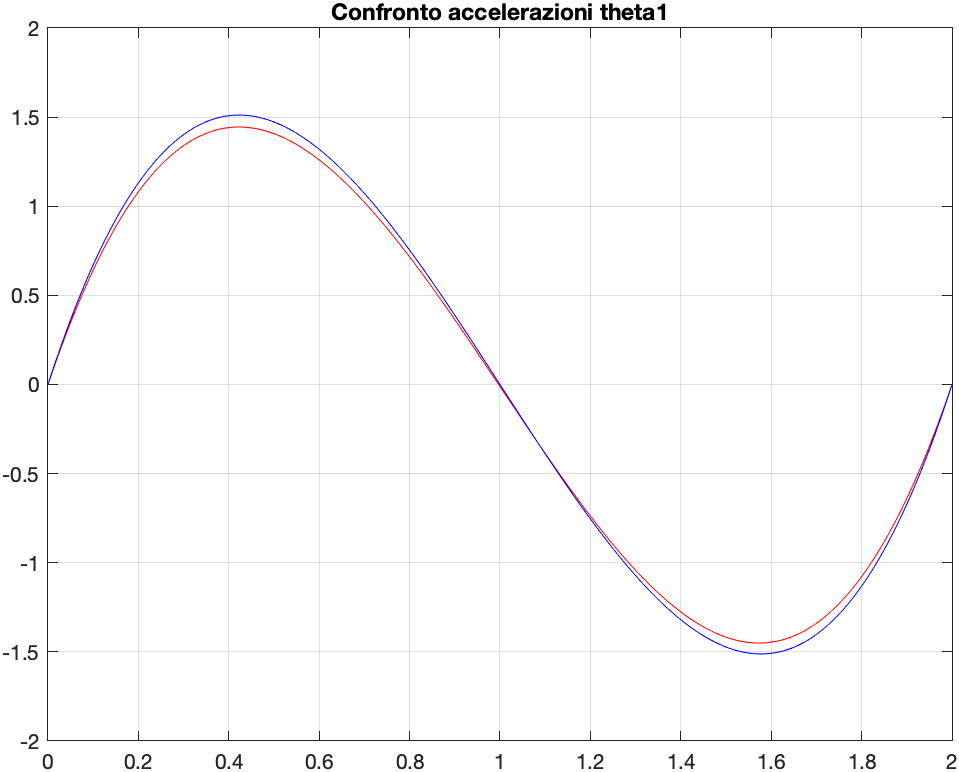
\includegraphics[width=.78\linewidth]{Immagini/Dinamica/confracct1.png}  
  \caption{Accelerazione $\theta_1$}
  \label{fig:sub-first}
\end{subfigure}
\begin{subfigure}{.45\textwidth}
  \centering
  % include second image
  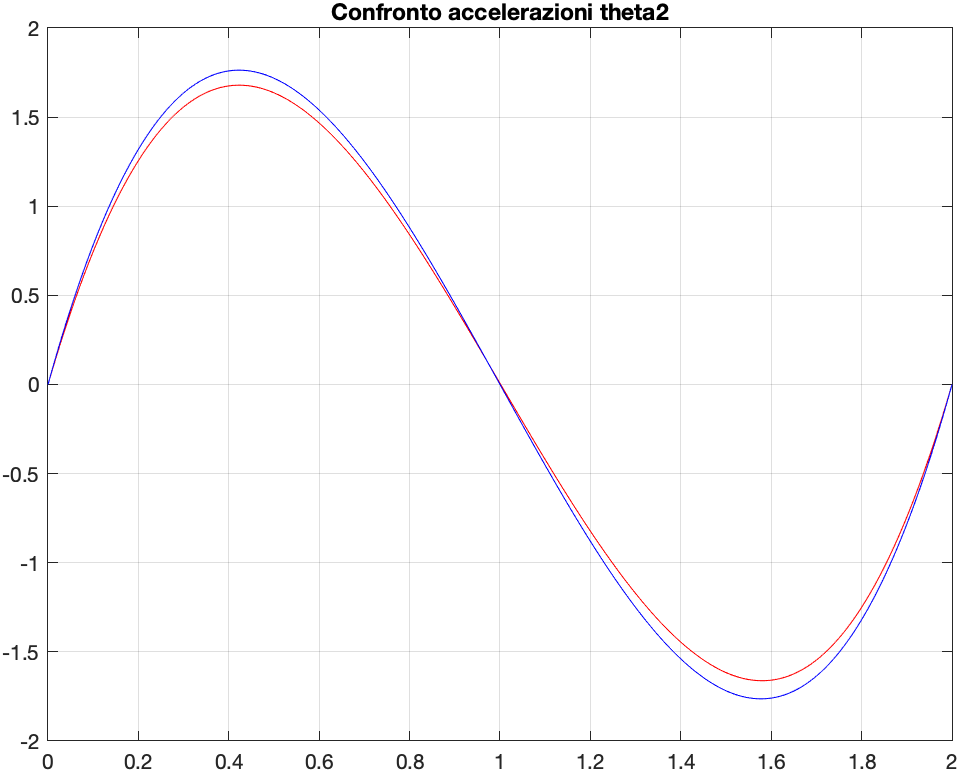
\includegraphics[width=.78\linewidth]{Immagini/Dinamica/confracct2.png}  
  \caption{Accelerazione $\theta_2$}
  \label{fig:sub-second}
\end{subfigure}
\caption{Confronto dinamica leggi di moto su accelerazioni}
\end{figure}
\begin{figure}[!ht]
\begin{subfigure}{.45\textwidth}
  \centering
  % include first image
  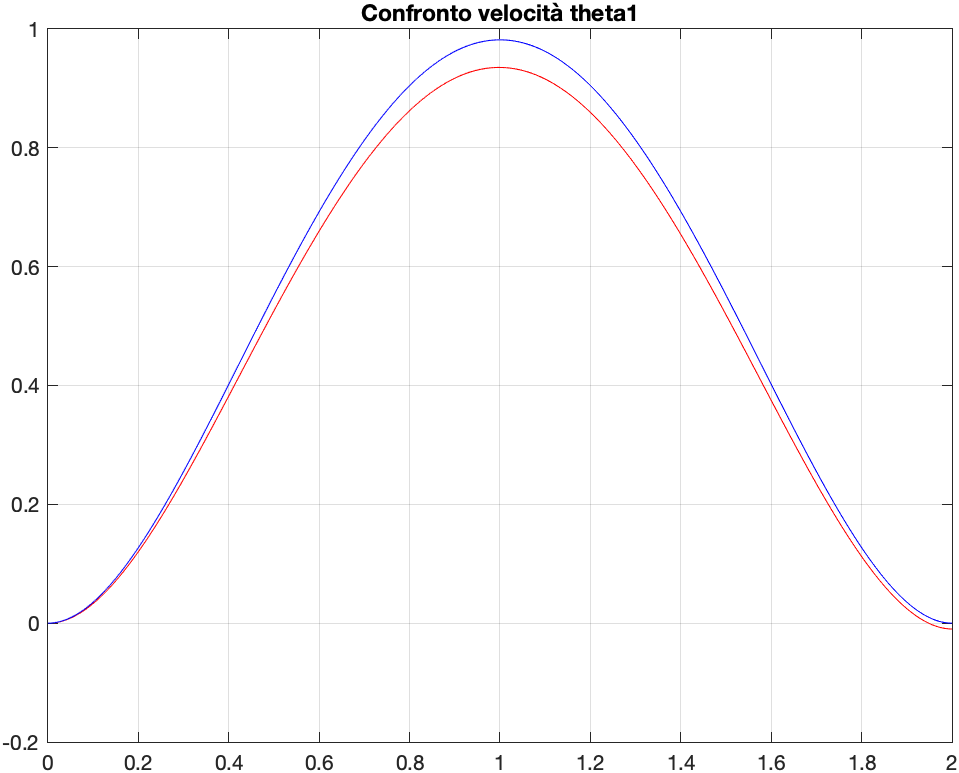
\includegraphics[width=.78\linewidth]{Immagini/Dinamica/confrvelt1.png}  
  \caption{Velocità $\theta_1$}
  \label{fig:sub-firstv}
\end{subfigure}
\begin{subfigure}{.45\textwidth}
  \centering
  % include second image
  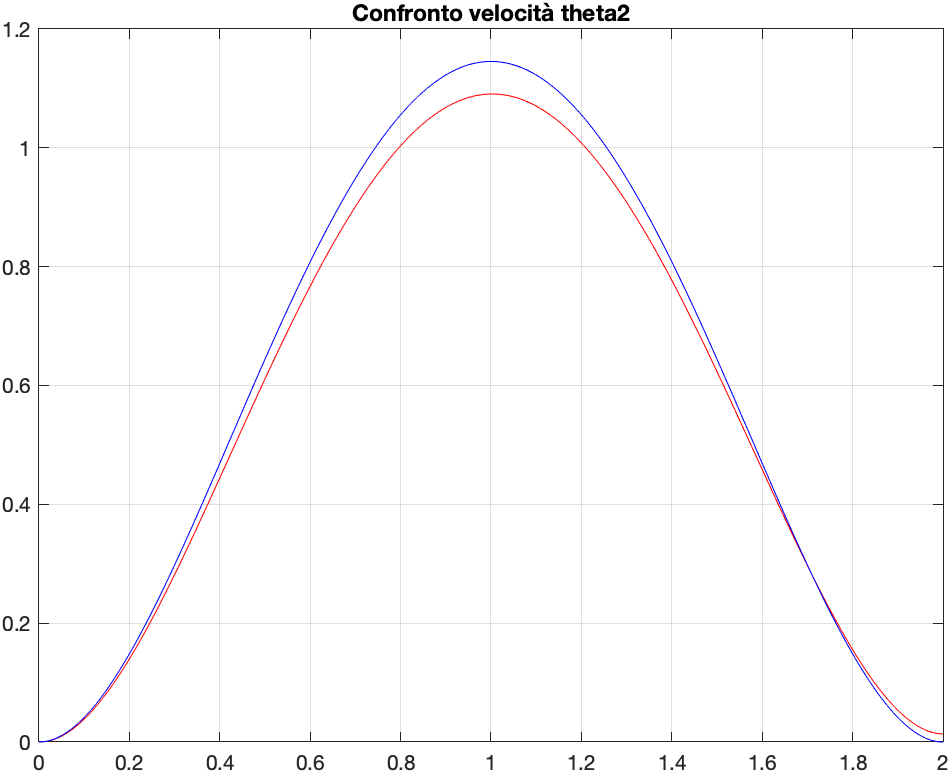
\includegraphics[width=.78\linewidth]{Immagini/Dinamica/confrtvelt2.png}  
  \caption{Velocità $\theta_2$}
  \label{fig:sub-secondv}
\end{subfigure}
\caption{Confronto dinamica leggi di moto su velocità}
\end{figure}
\begin{figure}[!ht]
\begin{subfigure}{.45\textwidth}
  \centering
  % include first image
  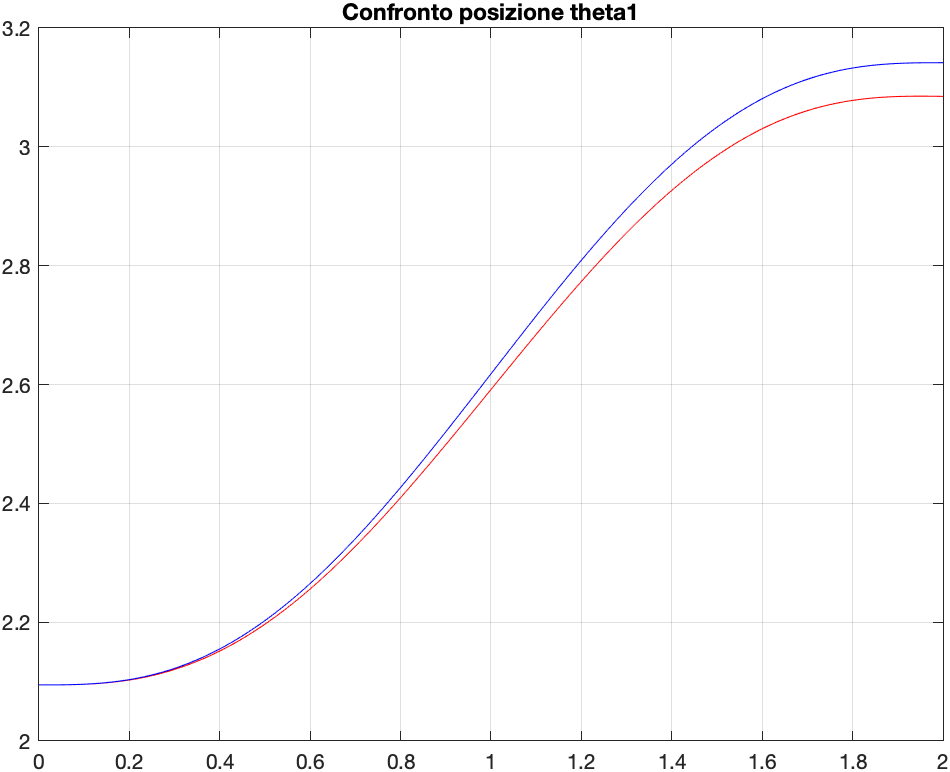
\includegraphics[width=.78\linewidth]{Immagini/Dinamica/confrpost1.png}  
  \caption{Posizione $\theta_1$}
  \label{fig:sub-firsta}
\end{subfigure}
\begin{subfigure}{.45\textwidth}
  \centering
  % include second image
  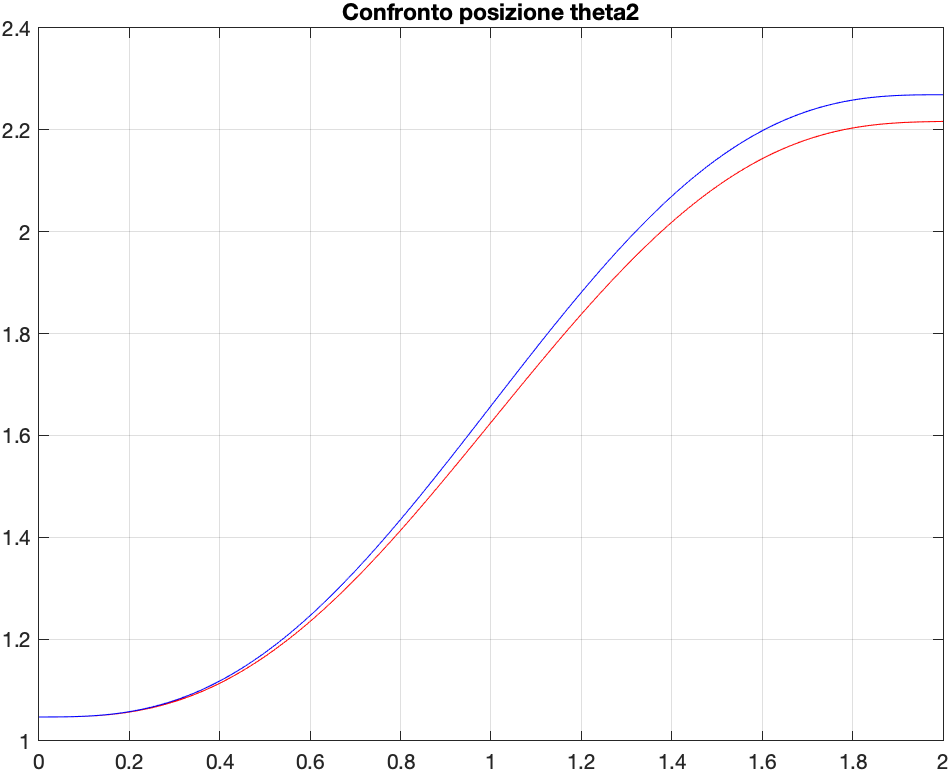
\includegraphics[width=.78\linewidth]{Immagini/Dinamica/confrpost2.png}  
  \caption{Posizione $\theta_2$}
  \label{fig:sub-seconda}
\end{subfigure}
\caption{Confronto dinamica leggi di moto su posizioni}
\end{figure}
Una volta calcolati tutti i parametri di nostro interesse andiamo a costruire il modello simulink che sarà utile per una visione d'insieme:
\begin{figure}[ht]
	\begin{center}
		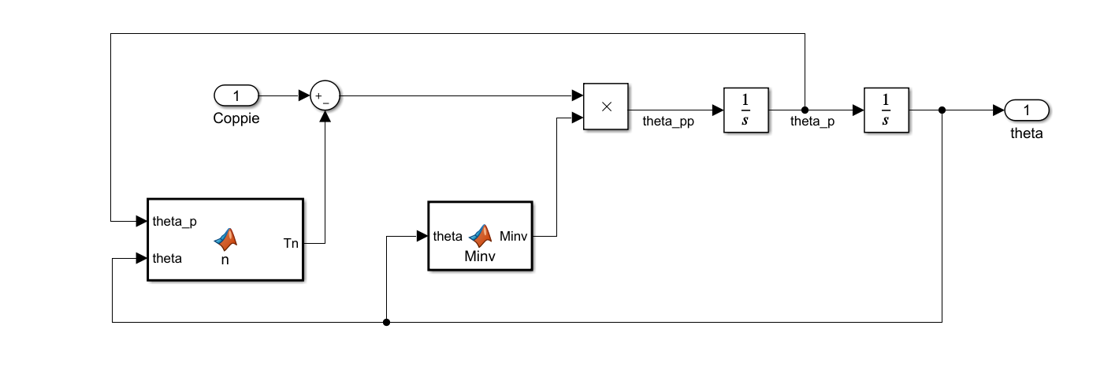
\includegraphics[scale=0.55]{Immagini/Dinamica/ModSimulink}
		\caption{Modello simulink manipolatore}
	\end{center}
\end{figure}
\subsubsection*{Modellazione su Adams}
\addcontentsline{toc}{subsubsection}{Modellazione su Adams}
Per quanto riguarda la modellazione su adams, è stato realizzato un prototipo del manipolatore composto da aste rigide, i due link motorizzati sono fissati mediante delle cerniere ed abbiamo anche la presenza dell'end-effector.
\begin{figure}[!ht]
	\begin{subfigure}{.5\textwidth}
		\centering
		% include first image
		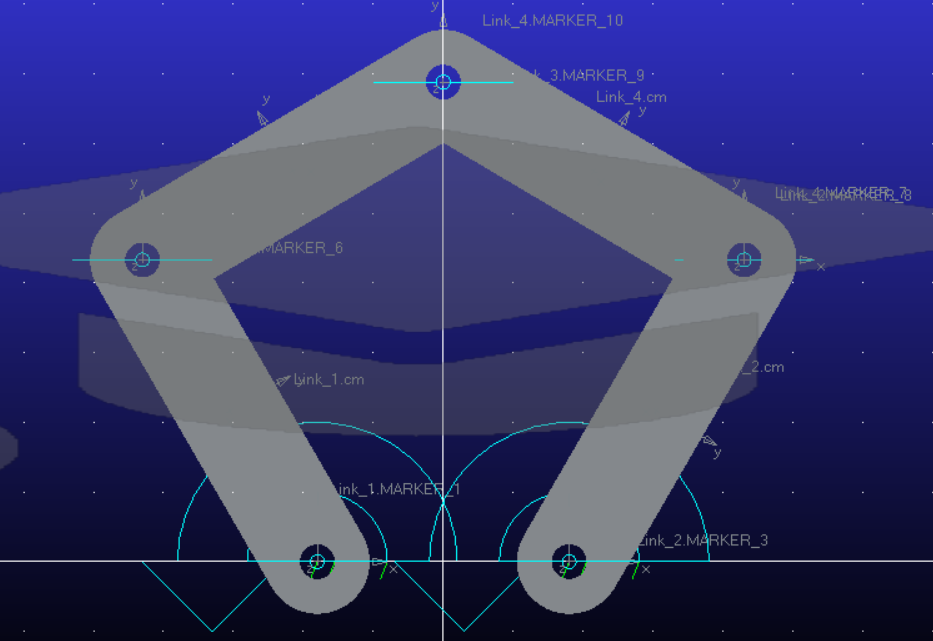
\includegraphics[width=.9\linewidth]{Immagini/Dinamica/adams1.png}  
		\caption{Vista dall'alto}
		\label{fig:sub-adams1}
	\end{subfigure}
	\begin{subfigure}{.5\textwidth}
		\centering
		% include second image
		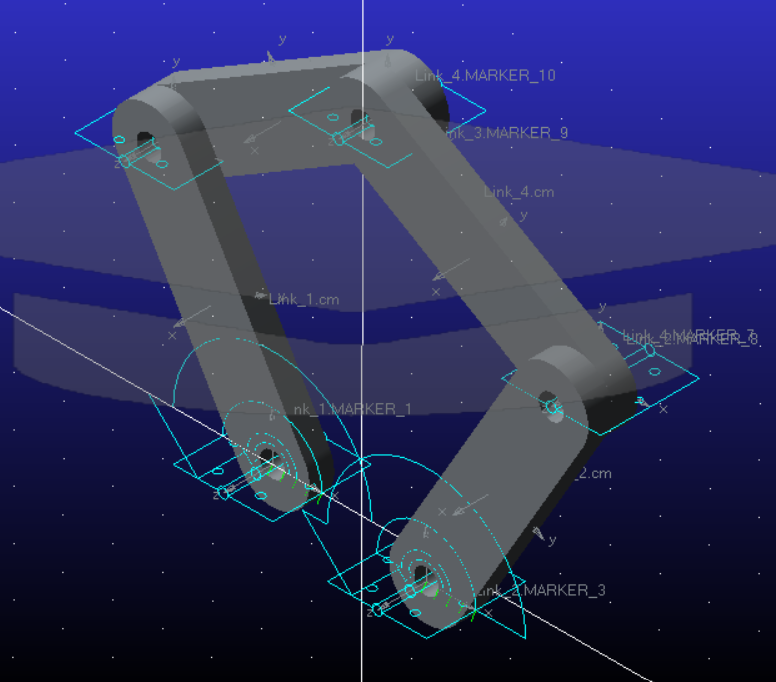
\includegraphics[width=.8\linewidth]{Immagini/Dinamica/adams2.png}  
		\caption{Vista in diagonale}
		\label{fig:sub-adams2}
	\end{subfigure}
	\caption{Modello Adams manipolatore 5R}
\end{figure}
Una volta definiti i vincoli e le modalità di movimento del manipolatore si è passati alla fase successiva ovvero quella dell'analisi del modello e della simulazione, andando ad assegnare leggi di moto al modello adams e verificare il suo comportamento rispetto al modello creato su simulink.
\subsubsection*{Validazione e confronto}
\addcontentsline{toc}{subsubsection}{Validazione e confronto}
Le leggi di moto assegnate al modello adams sono state anche assegnate nella stessa maniera al modello simulink, in particolare sono state utilizzate: 
\begin{table}[h!]
	\centering
	\begin{tabular}{|c|c|} 
		\hline
		Motore & Legge di moto  \\
		\hline\hline
		Motore 1 ($\theta_1$)& Sinusoidale $sin$ \\
		Motore 2 ($\theta_2$)& Sinusoidale $2\sin$ \\
		\hline
	\end{tabular}
	\caption{Leggi di moto validazione}
	\label{table:ldmAdams}
\end{table}
Una volta assegnata la legge ed eseguita la simulazione si è fatto un confronto:
\begin{figure}[!ht]
	\begin{subfigure}{.5\textwidth}
		\centering
		% include first image
		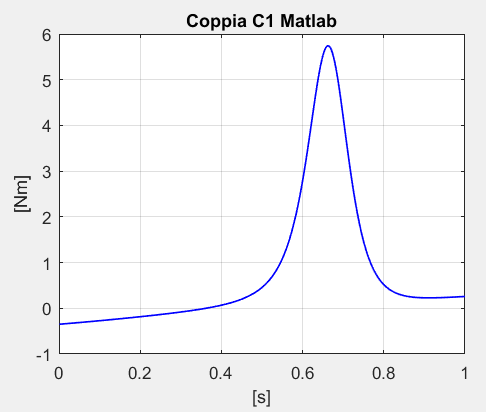
\includegraphics[width=.9\linewidth]{Immagini/Dinamica/c1matlab.png}  
		\caption{Coppia C1 Matlab}
		\label{fig:leggiC1M}
	\end{subfigure}
	\begin{subfigure}{.5\textwidth}
		\centering
		% include second image
		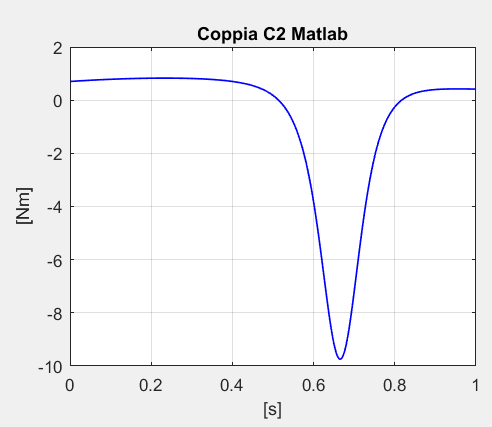
\includegraphics[width=.9\linewidth]{Immagini/Dinamica/c2matlab.png}  
		\caption{Coppia C2 Matlab}
		\label{fig:leggiC2M}
	\end{subfigure}
	\caption{Coppie in uscita Simulink}
\end{figure}
\begin{figure}[!ht]
	\begin{subfigure}{.5\textwidth}
		\centering
		% include first image
		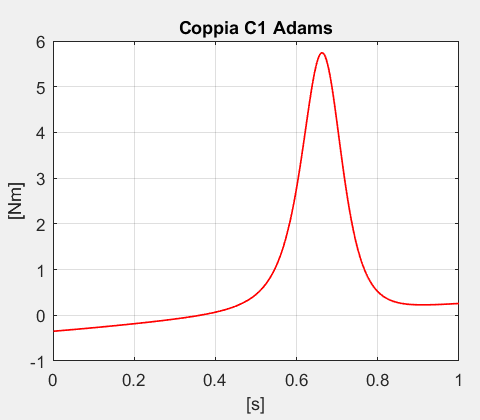
\includegraphics[width=.9\linewidth]{Immagini/Dinamica/c1adams.png}  
		\caption{Coppia C1 Adams}
		\label{fig:leggiC1A}
	\end{subfigure}
	\begin{subfigure}{.5\textwidth}
		\centering
		% include second image
		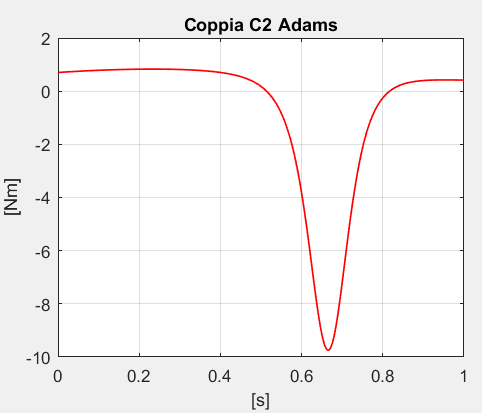
\includegraphics[width=.9\linewidth]{Immagini/Dinamica/c2adams.png}  
		\caption{Coppia C2 Adams}
		\label{fig:leggiC2A}
	\end{subfigure}
	\caption{Coppie in uscita Adams}
\end{figure}
Andando poi a fare una differenza tra questi due grafici riusciamo a trovare l'andamento dell'errore sulle coppie:
\begin{figure}[!ht]
	\begin{subfigure}{.5\textwidth}
		\centering
		% include first image
		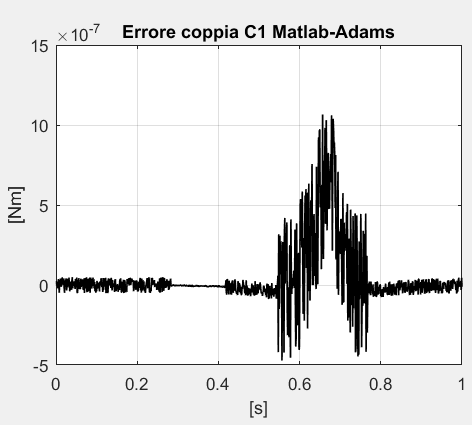
\includegraphics[width=.9\linewidth]{Immagini/Dinamica/confrc1.png}  
		\caption{Errore coppia C1}
		\label{fig:errC1}
	\end{subfigure}
	\begin{subfigure}{.5\textwidth}
		\centering
		% include second image
		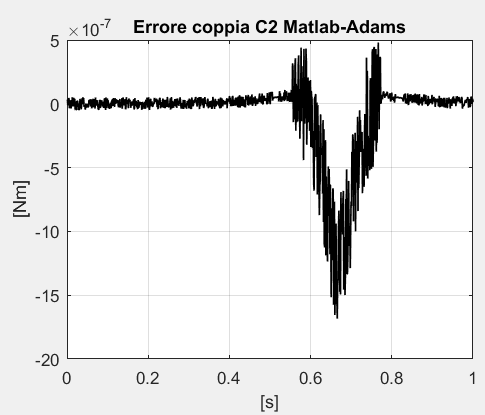
\includegraphics[width=.9\linewidth]{Immagini/Dinamica/confrc2.png}  
		\caption{Errore coppia C2}
		\label{fig:errC2}
	\end{subfigure}
	\caption{Errore Simulink-Adams}
\end{figure}
Analizzando il grafico vediamo che l'errore è nell'ordine di $10^{-7}$ di conseguenza è possibile vedere che la validazione ha portato un risultato positivo in quanto le coppie del modello Simulink e le coppie del modello Adams sono praticamente identiche a parte un fattore d'errore dato dalle diverse modalità di calcolo/integrazione.
\subsection{Punti di singolarità}
Nell'ambito matematico, una singolarità è un punto nel quale un oggetto non è definito, oppure un punto nel quale l'oggetto non ha un comportamento normale, nel nostro caso i punti di singolarità saranno punti che andranno a delimitare lo spazio di lavoro del robot. Definiamo spazio di lavoro del robot tutto un insieme di punti nei quali il robot ha un funzionamento normale e non presenta problematiche.\footnote{Passando per un punto di singolarità il robot potrebbe aver problemi che potrebbero causare anche la rottura di parti meccaniche} Andando a considerare la foto vista nell'introduzione, possiamo trovare sei casi di punti di singolarità, in particolare però non sono punti ma sono traiettorie. Di conseguenza il robot avrà come spazio di lavoro, tutto lo spazio che è interno (delimitato) da queste traiettorie.
\subsubsection*{Primo e secondo caso}
\addcontentsline{toc}{subsubsection}{Primo e secondo caso}
In questo primo caso abbiamo $\overrightarrow{CD}$ che è parallelo a $\overrightarrow{DE}$, schematicamente possiamo andarlo a rappresentare nel seguente modo
\begin{figure}[ht]
	\begin{center}
		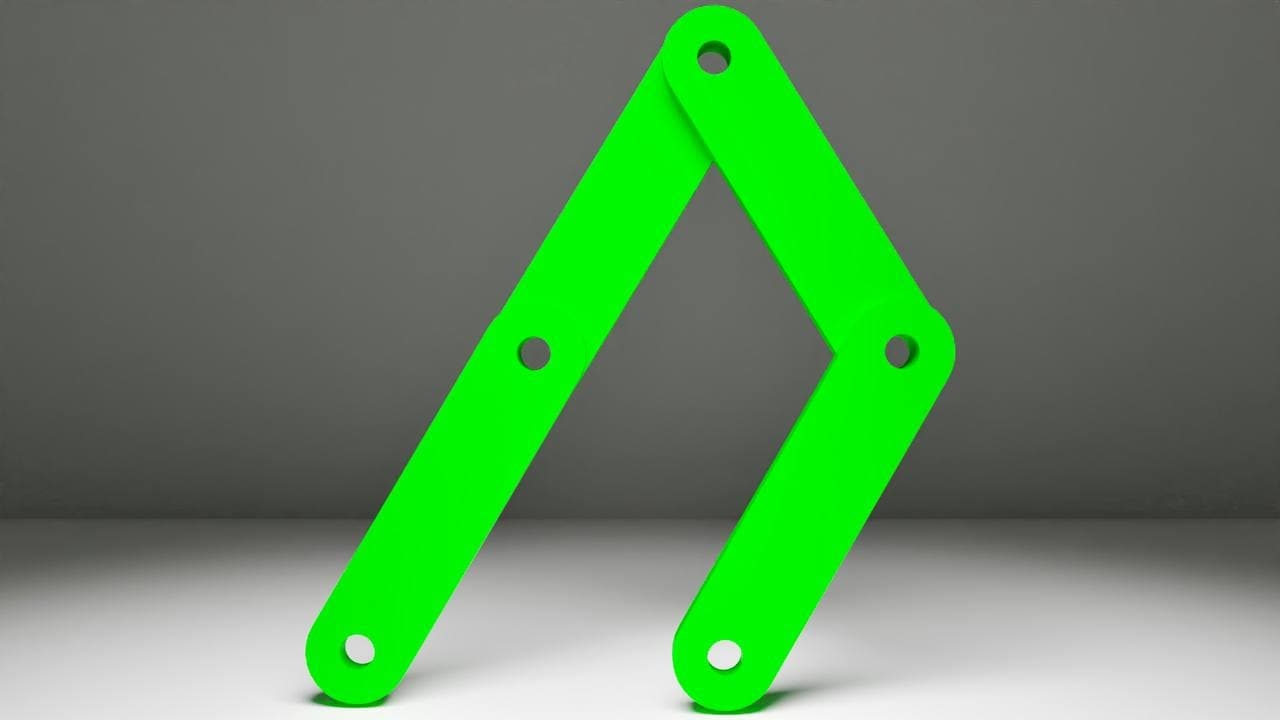
\includegraphics[scale=0.4]{Immagini/Singolarity/1}
		\caption{Caso 1 singolarità}
	\end{center}
\end{figure}
\\Lasciando la x libera possiamo ricavare la y come:
\begin{equation}
    y_1 = \sqrt{4l^2-(x-d)^2}
\end{equation}
Per quanto riguarda il secondo caso è molto simile al primo, la differenza sta nel fatto che abbiamo la catena $\overrightarrow{AB}$ parallela a $\overrightarrow{BC}$ 
\begin{figure}[ht]
	\begin{center}
		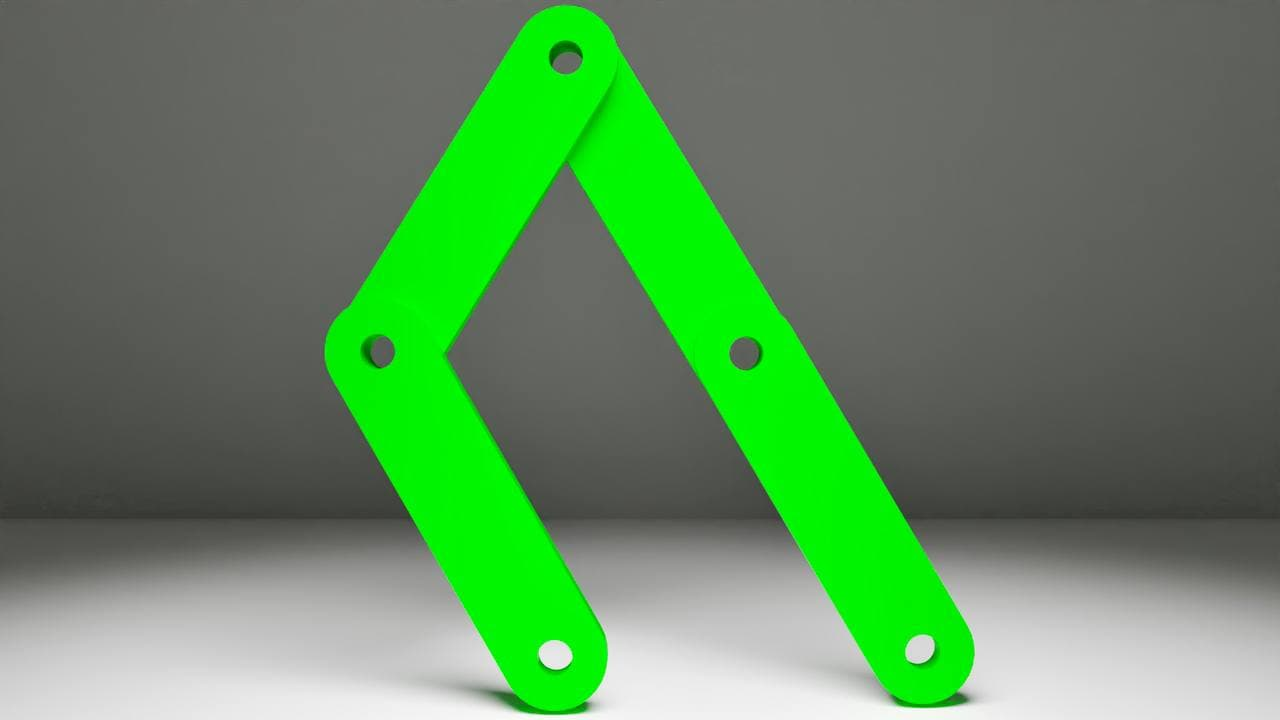
\includegraphics[scale=0.4]{Immagini/Singolarity/2}
		\caption{Caso 2 singolarità}
	\end{center}
\end{figure}
Il procedimento è simile a prima, lasciando sempre la x libera possiamo trovare la y come:
\begin{equation}
    y_2 = \sqrt{4l^2-(x+d)^2}
\end{equation}
Entrambi i casi producono come risultato una circonferenza.
\subsubsection*{Terzo caso}
\addcontentsline{toc}{subsubsection}{Terzo caso}
Il terzo caso di singolarità avviene quando i due link non motorizzati sono paralleli, questa configurazione aggiunge un grado di libertà al sistema, in quanto l'end-effector per muoversi ha necessità di una maggior coppia per riuscire a superare la situazione di stallo
\begin{figure}[ht]
	\begin{center}
		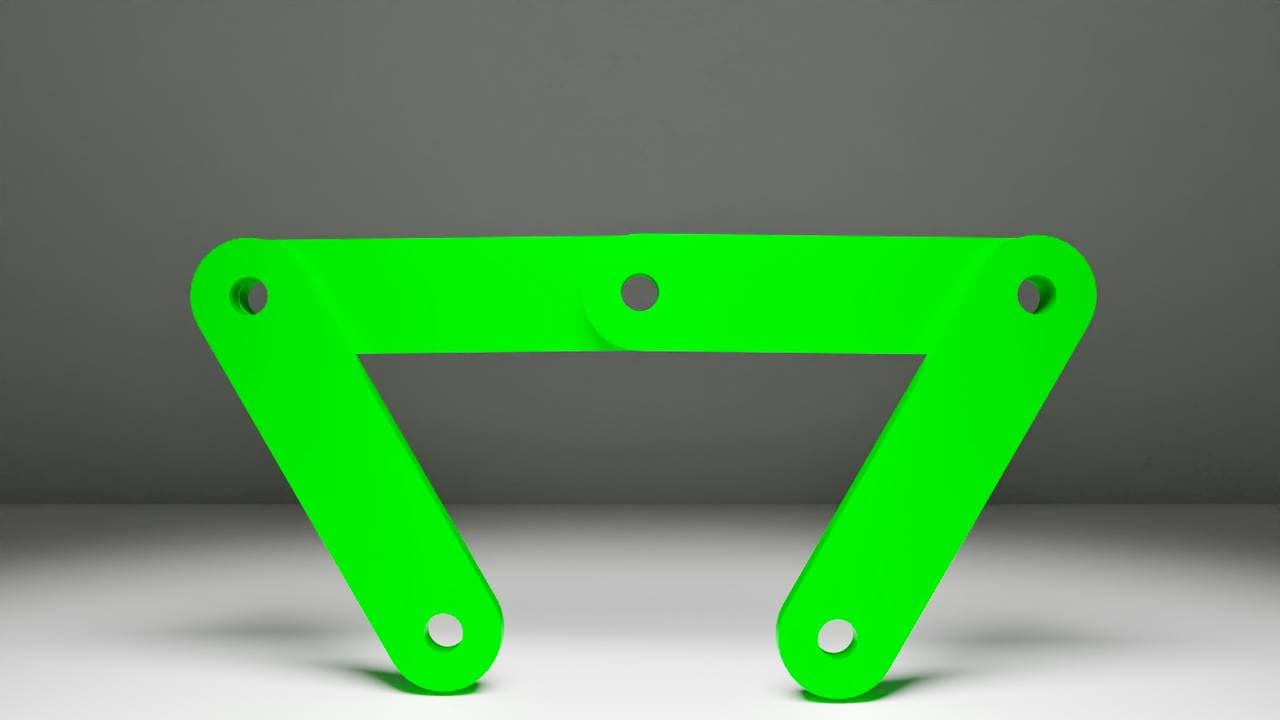
\includegraphics[scale=0.4]{Immagini/Singolarity/5}
		\caption{Caso 3 singolarità}
	\end{center}
\end{figure}
\\Per quanto riguarda la soluzione, andiamo a considerare $\theta_1$ che varia da 0 a $360^\circ$ e andiamo a cercare le coppie di valori $[x,y]$ relative alla singolarità. Uscirà un'equazione di secondo grado, con i seguenti coefficienti:
\begin{equation*}
	a = l^2\sin^2\theta_1 + 4d^2-4dl\cos\theta_1 + l^2\cos^2\theta_1
\end{equation*}
\begin{equation*}
	b = 2l^3\sin\theta_1 + 2dl^2\sin\theta_1\cos\theta_1-2dl\sin\theta_1(2d-2l\cos\theta_1)
\end{equation*}
\begin{equation*}
	c = l^2(l^2+d^2\cos^2\theta_1+2ld\cos\theta_1)-2dl(l+d\cos\theta_1)(2d-l\cos\theta_1)+d^2-l^2(2d-l\cos\theta_1)^2
\end{equation*}
Risolviamo l'equazione di secondo grado:
\begin{equation*}
	\Delta = b^2-4ac
\end{equation*}
Andiamo a trovare le radici y di quest'equazione, definendo poi: $sx = -b+l\cos\theta_1$ ed $sy = l\sin\theta_1$ possiamo andare a trovare le soluzioni dell'equazione come:
\begin{equation}
	x_3 = \bigg|\frac{x_{3p}+sx}{2}\bigg|, y_3 = \bigg|\frac{y_{3p}+sy}{2}\bigg|
\end{equation}
Con 
\begin{equation*}
	x_{3p} = \frac{l^2+y_{3p}l\sin\theta_1+ld\cos\theta_1}{2d-l\cos\theta_1}
\end{equation*}
\subsubsection*{Quarto e quinto caso}
\addcontentsline{toc}{subsubsection}{Terzo e quarto caso}
Il quarto e quinto caso sono casi di singolarità non realizzabili nella pratica, ma sono di interesse teorico. Il primo caso prevede che la posizione dell'end-effector coincida con la posizione del primo giunto motorizzato e nell'altro caso coinciderà con il secondo giunto motorizzato. Come soluzioni avremo semplicemente due punti e possiamo andare a calcolarli nei seguenti modi:
\begin{figure}[!ht]
	\begin{subfigure}{.5\textwidth}
		\centering
		% include first image
		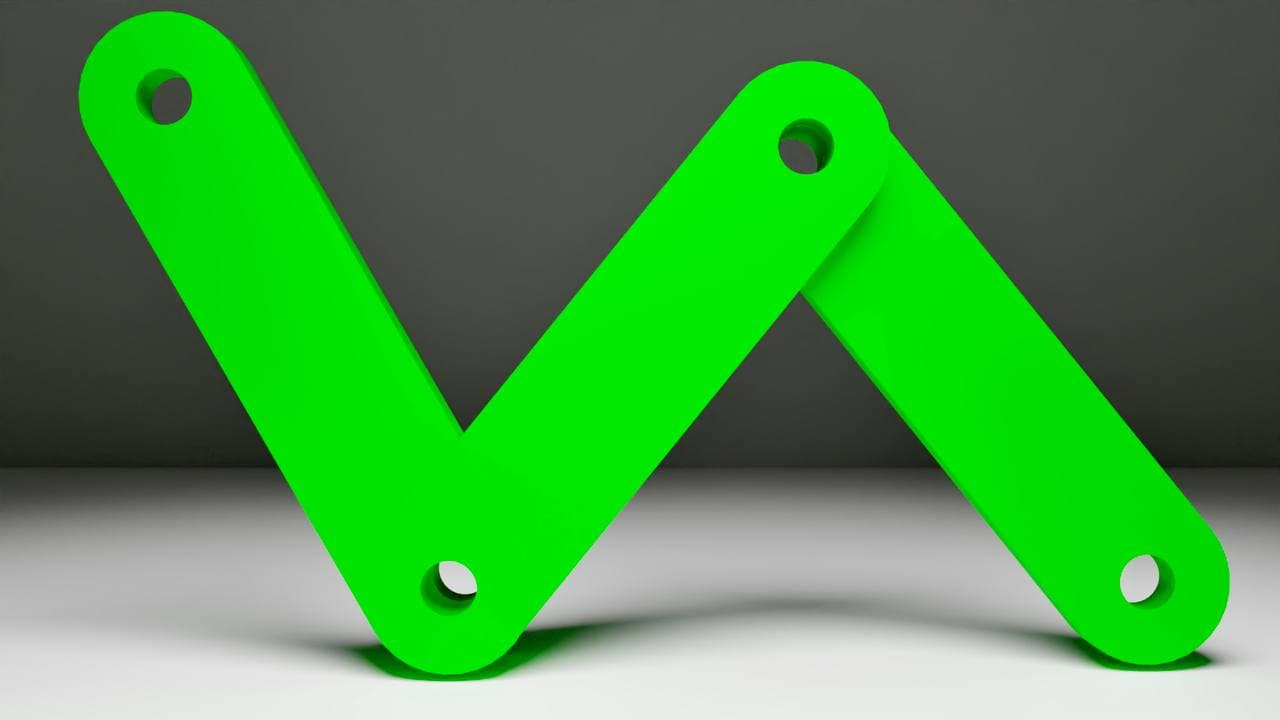
\includegraphics[width=.9\linewidth]{Immagini/Singolarity/3}
		\label{fig:sing4}
	\end{subfigure}
	\begin{subfigure}{.5\textwidth}
		\centering
		% include second image
		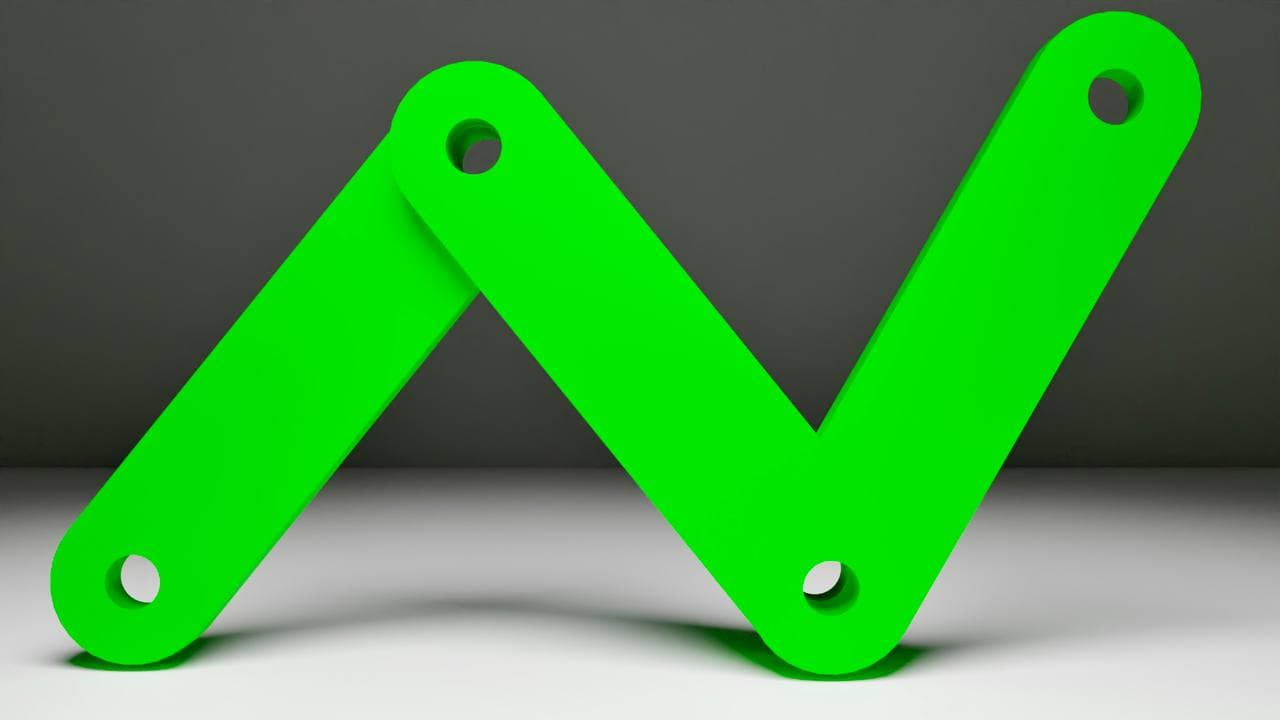
\includegraphics[width=.9\linewidth]{Immagini/Singolarity/4}  
		\label{fig:sing5}
	\end{subfigure}
	\caption{Caso 4 e 5 singolarità}
\end{figure}
Le soluzioni le possiamo trovare impostando che la lunghezza della x vale nel quarto caso d e nel quinto -d, andando quindi a trovare le soluzioni come:
\begin{equation}
    y_4 = \sqrt{-(x-d)^2}
\end{equation}
e
\begin{equation}
    y_5 = \sqrt{-(x+d)^2}
\end{equation}
Andando ad unire tutti casi visti fino ad ora possiamo vederli visualmente nell'asse $[x,y]$
\begin{figure}[ht]
\begin{center}
    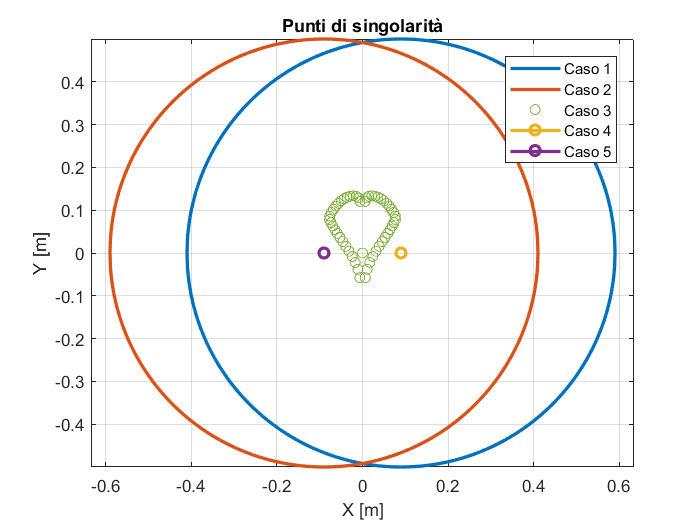
\includegraphics[scale=0.65]{Immagini/Singolarity/SingNew}
    \caption{Punti di singolarità}
\end{center}
\end{figure}
\subsection{Manipolabilità}
La manipolabilità ci permette di avere una rappresentazione geometrica delle capacità che ha un punto del nostro sistema. Per andare a calcolarla abbiamo bisogno dell'equazione \ref{eq:J12}, vista nella sezione \ref{sec:CalcoloVelCin}.
\\Andiamo a definire la matrice
\begin{equation}
    J_{man} = JJ^T
\end{equation}
Da questa possiamo ricavare gli autovalori $\Lambda$. Definiamo poi  l'indice di manipolabilità \textbf{r} come:
\begin{equation}
    r = \frac{\max\lambda}{\min\lambda}
\end{equation}
Questo numero può variare tra 1 e $+\infty$, più è piccolo e meno si rischia di andare in singolarità. Possiamo andare a rappresentare il numero di condizionamento tramite i grafici seguenti: 
\begin{figure}[!ht]
	\begin{subfigure}{.55\textwidth}
		\centering
		% include first image
		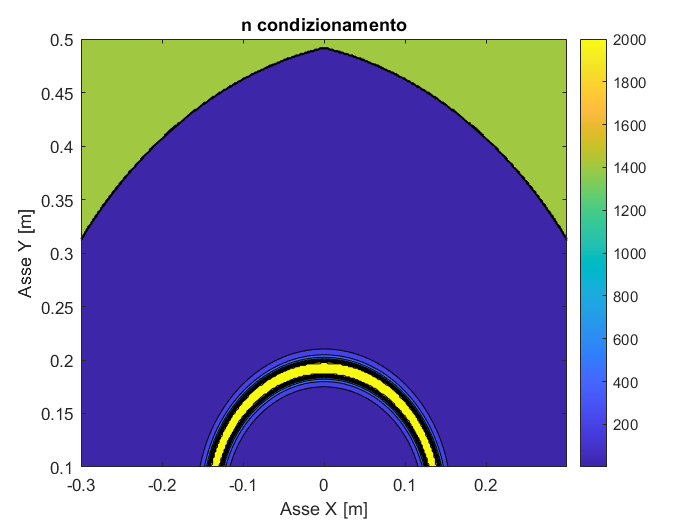
\includegraphics[width=.9\linewidth]{Immagini/Singolarity/Ncond}
		\label{fig:ncond}
	\end{subfigure}
	\begin{subfigure}{.55\textwidth}
		\centering
		% include second image
		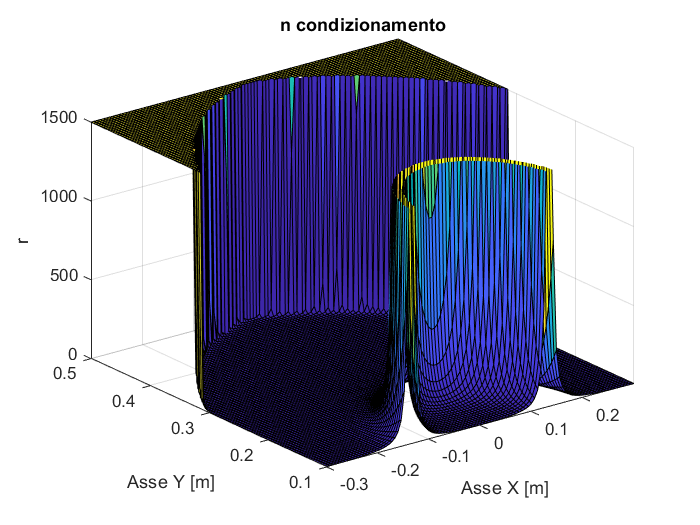
\includegraphics[width=.9\linewidth]{Immagini/Singolarity/Ncond_surf}  
		\label{fig:nconds}
	\end{subfigure}
	\caption{Numero di condizionamento}
\end{figure}
\\Nel primo grafico viene mostrato il piano x,y ed il numero di condizionamento è definito come una colormap, i punti di color blu sono quelli con un r piccolo ed in questi non siamo in condizioni di singolarità, invece quelli tendenti al verde/giallo sono i casi di singolarità che abbiamo visto prima. Nella seconda figura abbiamo la stessa rappresentazione però in tre dimensioni, utilizziamo l'asse z per rappresentare il numero di condizionamento; anche qua le zone di singolarità sono chiaramente visibili.
In questo secondo grafico invece andiamo a concentrarci sulla zona di movimentazione ideale del manipolatore, più ci si avvicina allo zero, più il valore di r aumenta, questo per il fatto che stiamo raggiungendo una zona di singolarità.
\subsection{Workspace}
Dalle analisi appena effettuate sui punti di singolarità e sul numero di condizionamento è stato possibile descrivere lo spazio di lavoro del manipolatore.
\begin{figure}[ht]
	\begin{center}
		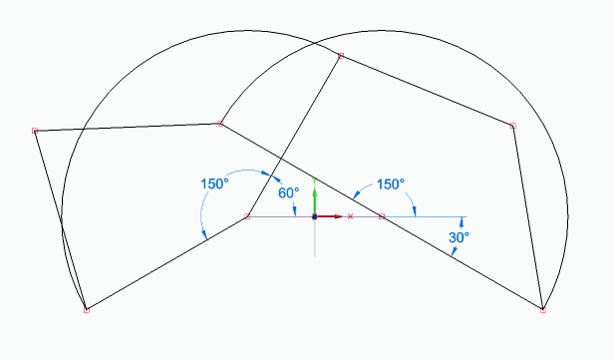
\includegraphics[scale=0.5]{Immagini/Singolarity/workangle}
		\caption{Angoli di movimentazione dei giunti motorizzati}
	\end{center}
\end{figure}
Unendo poi gli angoli di movimentazione del manipolatore, è stato possibile descrivere lo spazio di lavoro mediante un rettangolo inscritto che non viola i punti di singolarità
\begin{figure}[ht]
	\begin{center}
		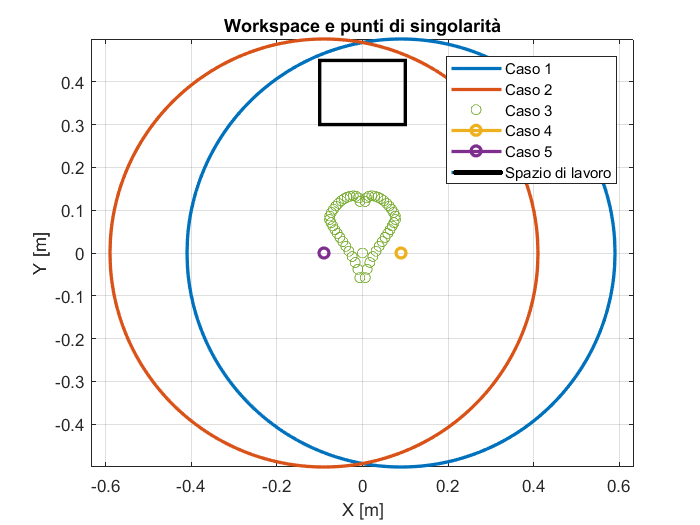
\includegraphics[scale=0.5]{Immagini/Singolarity/Worksing}
		\caption{\textit{Workspace} 5R}
	\end{center}
\end{figure}
\\In particolare è stata anche fatta un'analisi sul numero di condizionamento del \textit{workspace}:
\begin{figure}[ht]
	\begin{center}
		\includegraphics[scale=0.5]{Immagini/Singolarity/ncondsl}
		\caption{Numero di condizionamento workspace}
	\end{center}
\end{figure}
Su tutto il piano x,y si nota come il numero di condizionamento assume valori bassi, questo implica che non vi è singolarità, gli unici punti critici sono quelli esterni, nei quali il valore è vicino a 6, (comunque minore di $\infty$), questi punti vanno a rappresentare casi nei quali il manipolatore avrà più difficoltà a muoversi, ma non sono veri e propri casi di singolarità .